\documentclass[../main/main.tex]{subfiles}

\newdate{date}{26}{03}{2020}



\begin{document}

\section{Lecture 6}
\displaydate{date}. Compiled:  \today. Alice.


\subsubsection{Slide 90}

\begin{figure}[h!]
\centering
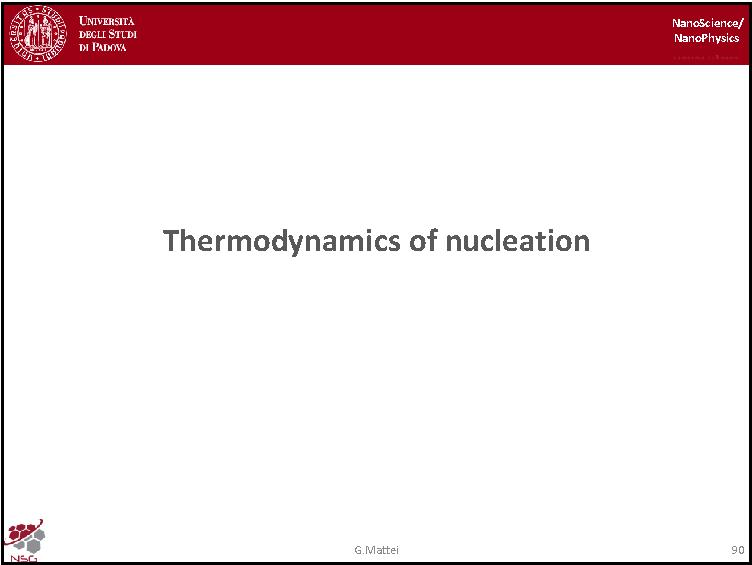
\includegraphics[page=1,width=0.9\textwidth]{../lessons/pdf_file/6_lesson.pdf}
\end{figure}


In the previous lecture we have seen how to experimentally verified the concept which are the base of theromydnamic size affect and how the interaction between the matrix and nanoparticles can affect the entire process through as for instance a mechanical force as the idrostatic pressure around the nanoparticle. When you control the size of the nanoparticles you can control his properties and the thermodynamic size effect is a clear manifestation of this pecular control of size dependent property at the nanoscal as the melting temperature.

Another interesting problem is the physics of the basis of nucleation. How we can control nucleation ang use a botton/up approach in which we obtain nanoparticles by an ensemble of atoms basically. This could be in a vapour phase, liquid or solid phase. We need to resort the basic thermodynamic of nucleation and this will be the subject of this lesson.

\newpage
\subsubsection{Slide 91}

\begin{figure}[h!]
\centering
\includegraphics[page=2,width=0.9\textwidth]{../lessons/pdf_file/6_lesson.pdf}
\end{figure}

If you want to sinthesize nanostructure materials you can resort very different set of techniques. In this slide those techniques are recapped, divided into physical and chemical. Of course, these division is strong, because normally the techniques involse both chemical and physical effects, so a classification is meaningful, but just to have a raw picture we can divide it into these two class.

We have:
\begin{itemize}
\item \textbf{Physical techniques}.
\begin{itemize}
\item \textbf{Condensation from vapour phase}. We have seen in the case of led nanoparticles condensed on the silica substrate to produce the nanoparticles we have seen.
\item \textbf{Free expansion} (Molecular beam expansion techniques).
\item \textbf{Sputtering} (Physical vapor deposition).
\item \textbf{Ion implantation}.
\item \textbf{Ball-milling}. It is a top/down techniques, tou start from a polders and you try to reduce the side by interaction with spheres which are able to meal the polders and reduce its size due to strong interactions during the collision between the balls.
\item \textbf{Lithography, Nanofabrication}. It can be electronical lythography, optical one, or X-Ray...there are a lot of such kind of properties.
\item \textbf{Laser ablation}. You vaporize solid and you collect either in liquid or in vacuum the evaporated atoms at the surface locally.
\end{itemize}
Those are the techniques which characterize physical proecesses: energy transfer from the source to a target which produce the atoms which then are used to produce the nanostructures.
\item \textbf{Chemical techniques}.
\begin{itemize}
\item \textbf{Collaidal chemistry}. Based on the fact that you can produce out something that you decompose and precipitate under controlled conditions.
\item \textbf{Sol-gel}. For producing thin film of nanoparticles, you start from the solution then you condensate through suitable chemical and thermal processes.
\item \textbf{Standard chemical vapor deposition}. It is similar to the physical sputtering but instead of using the interaction of the plasma with the solid target to produce the atoms, you normally decompose some chemical precorses and then let the product of those chemical precourses to deposit and to form the nanostructure.
\end{itemize}

\end{itemize}
Normally you can have mixed approach, this just a very rough classification.

I would like to discuss the basic mechanicsm underlying these techniques: in particular all of these are based on the bottom/up approach (we exlude Ball-milling and lithography). All these techniques are based on the concept of \textbf{supersaturation}

\newpage
\subsubsection{Slide 92}

\begin{figure}[h!]
\centering
\includegraphics[page=3,width=0.9\textwidth]{../lessons/pdf_file/6_lesson.pdf}
\end{figure}

If we go for the classical theory of nucleation (we give just a hint of basic concepts). \textbf{Nucleation} normally occur when a phase is dispersed into a solvent and then if the concentration is sufficiently large or if you have defects in the environment you can start nucleating embrios of the new phases which trigger the  subsequent grows of the nanostructures.

Nucleation can be divided into:
\begin{itemize}
\item \textbf{Homogeneous} nucleation. Involves just pure faces, with no defects. If you think about of the condensation of a droplet in the presence of a vapour and nothing else we can think about homogeneous nucleation.
\item \textbf{Heterogeneous} nucleation constitute the majority of cases. It involves the present of defects that act as sites for promoting nucleation, hence the energy barrier that you need to pass for obtaining in the case of heterogeneous nucleation, those energy barriers are lowered by the presence of defects, which are a sort of catalitic sites for precipitation.
\end{itemize}
In the following, we will use the simplifying hypothesis that the nucleating embryos are just spherical droplets. This is a quit useful approximation, because it allows to use macroscopic thermodynamic properties for all the quantities that we will need to obtain numerical evaluation of the quantities of interest. It is the same approximation that we used for the theromydnamic size effect.

\newpage
\subsubsection{Slide 93}

\begin{figure}[h!]
\centering
\includegraphics[page=4,width=0.9\textwidth]{../lessons/pdf_file/6_lesson.pdf}
\end{figure}

Suppose that we want to find the thermodynamic of the nucleation, so for instance the liquid phase out of vapor phase, which can be used as the prototipe for describing the nuleation, even if we are in presence of defects (heterogeneous nucleation), provided that we will lower all the energy barrier that we will see. Let us suppose this kind of system, liquid phase out of vapor phase, a quantity that we may want to calculate for nucleation is the variation of Gibbs free energy that is the, reversible work that we do on the system to create a unit surface between the liquid and the vapor phase \( \Delta G \). We can express this as a function of the atoms or of the radius in the nucleated phase. In both cases, we can express this Gibbs free energy variation by two contribution: one coming from the volume of the droplet (the terms that are negative, they tend to decrease the variation and tend to stabilize the entire system) while the other term has a positive sign and is related to the creation of the surface. The latter will tend to destibilize the system.

Of course, the term \( 4 \pi R^2 \gamma   \) will dominate at lower value of the radius of the droplated while the \( - \frac{4 \pi }{3} R^3 \delta g_v \) will dominate for larger value. So they stabilize toward the bulk the system that will precipitate.

If we want to write these function as a function of the temperature and of other input quantities that we may need to control to obtain a controlled nucleation in our system. We can use the Gibbs-Thompson equation. We obtain formula (1) which has a logartihm of the \( P^* \), that is the ration between the pressure at which we can produce the nucleating face normalized to the vapor pressure (pressure at which at a given temperature, the liquid and the vapor are in quilibrium as bulk faces). In particular, \( P_e \) is a function of temperature and so we can control the degree of supersaturation by adding atom on the vapor phase or by decreasing the temperature (that is decreasing the vapor pressure in the system). This \( P^* \) ratio is called \textbf{degree of super-saturation}. If it is larger than 1, the term \( -N \Delta g_N \) will be normally negative and it will help stabilizing the structure. If it is less than one we are in \textbf{under-saturation} and we will have that the factor is positive and it will destabilize the system, so it will breaks the nucleating embryos.

As far as the surface, we can equate the two expression and we can compute what is the contribution of the surface in the case of express as a function of \( N \), and we can obtain a link between the two description by \( R=R_0N^{1/3} \), which correlates the radius of the nucleated embryos to the number of atoms in that droplets as a function of the atomic radius \( R_0 \).

We end up with this description of the Gibbs free energy (2).

\newpage
\subsubsection{Slide 94}

\begin{figure}[h!]
\centering
\includegraphics[page=5,width=0.9\textwidth]{../lessons/pdf_file/6_lesson.pdf}
\end{figure}

If we plot the two curves, basically we end up in this two evolutions. The curve in the left has a maximum which can be calcuated by the derivative of the Gibbs free energy with respect to \( R \) (or \( N \)). We find the \( R^* \) and \( N^* \), radius of critical nucleus and number of atoms in the critical nucleus.
If we calculate those value of the maximum, we can calculate the respectively variation of the Gibbs free energy which corresponds to the barrier in energy that we need to overcome to obtain stabilization of the precipitated phase with respect to the solved atom in the system.
This is the barrier that is lowered when we have Heterogeneous nucleation.


\newpage
\subsubsection{Slide 95}

\begin{figure}[h!]
\centering
\includegraphics[page=6,width=0.9\textwidth]{../lessons/pdf_file/6_lesson.pdf}
\end{figure}


If we compute those quantities we will see that \( R^* \) it directly proportional to \( \gamma   \) and inverse proportional to \( \ln{ P^*} \), which means we can obtain easier stabilization when the degree of supersaturation is larger.
For instance when we have calculated \( N^* \) and \( R^* \), we can calculated the height of the barrier that we need to pass to obtain stabilization of our system \( \Delta G (N^*) \). You see that you can lower this heigh by increasing the temperature or the degree of superasturation.

Another interesting quantity is the \textbf{nucleation rate} \( J \), which of course is in the typical exponential form in which we have the barrier that we need to overcome normalized by the boltzmann factor (dependence on the temperature), and multiplied a preexponential factor which takes into account all the other quantities in the theory. What is important is the dependence on the temperature of both the \( \Delta G \), the critical value of the barrier, and \( K_B T \).

\newpage
\subsubsection{Slide 96}

\begin{figure}[h!]
\centering
\includegraphics[page=7,width=0.9\textwidth]{../lessons/pdf_file/6_lesson.pdf}
\end{figure}

One of the most important concept which is useful for understanding the basic phenomena occurring at the nanoscale whe you want to nucleate, growth and to control the growh of nanoparticle is the \textbf{Gibbs-Thomdon equation}.

\newpage
\subsubsection{Slide 97-98-99}

\begin{figure}[h!]
\centering
\includegraphics[page=8,width=0.9\textwidth]{../lessons/pdf_file/6_lesson.pdf} 
\end{figure}
\begin{figure}[h!]
\centering
\includegraphics[page=9,width=0.9\textwidth]{../lessons/pdf_file/6_lesson.pdf} 
\end{figure}
\begin{figure}[h!]
\centering
\includegraphics[page=10,width=0.9\textwidth]{../lessons/pdf_file/6_lesson.pdf}
\end{figure}

Suppose that we are working  at the given temperature (fixed for what we want to investigate) and we want to calculate which is the pressure of the vapor at which at that given temperature \( T \) a liquid droplet is in equilibrium with the vapor. That is, if we are considering a bulk liquid face in equilibrium with its vapor at that specific temperature, the pressure at which the two faces are in equilibrium is by definition the vapor pressure of that specific element. If instead we substitute this bulk liquid with a nanostructure liquid, if we want to nucleate a droplet of that liquid out of the vapor, we are interested in calculating the pressure at which the two system are in equilibrium at the very same temperature \( T \).

For doing that we basically want to transform the system number (1) to the system number (2) at a fixed temperature. So we will start by transforming the vapor at that specific pressure \( P_e \), to a vapor at a new pressure \( P(R) \) (dependent on the size of nanoparticle), then we want to transform the liquid at the pressure \( P_e \) to the pressure \( P(R) \).  The bulk liquid at the new pressure is transformed into a droplet of the same liquid at the new pressure. We will see all those three steps combining them and we will evaluate the variation of the chemical potential in the three steps. We will obtain the value of the new size dependent vapor pressure \( P(R) \) at a specific temperature for a droplet of liquid in equilibrium with its vapor at that specific temperature.


\begin{enumerate}
\item Let us start with the first transformation: we want to transform a vapor to one pressure to another one. In the following we will obtain \( P(R)>P_e \). For the moment let us assume two different pressure and we do the transformation of the vapor at constant temperature. We can use the very simple model of a perfect gas for computing this tranaformation. We use the definition of the Gibbs free energy \( G \) and we do an infinitesimal transformation at a constant temperature obtaining \( \dd[]{G}  \).
If we consider that we are working at isothermal condition \( \dd[]{T}=0  \). Then we compute \( \Delta G \) from going from \( P_e \) to \( P(R) \).
We can compute the difference of the chemical potential \( \Delta \mu  \). This is easy for the ideal gas approximation.
\item The other simple tranformation is: can we compress (or change) the pressure in the bulk liquid? What is the different in the chemical potential? We resort to the incrompressibility of the liquids, if we change the pressure there is no compression in the liquid so basically its thermodynamic chemical potential will stay the same. Their difference is negligible.

At this point we have vapor \( V \) and the liquid in the bulk \( L \) at this new pressure. Then we need to do the final transformation and compare the variation in the Gibbs free energy by transforming the bulk liquid into a droplet of the liquid at the same temperature and at this pressure.

\item  We can simply resort to the evaluation of the Gibbs free energy variation when we want to nucleated and growth a cluster of radius \( R \) at the nw pressure \( P(R) \). The cluster is in equilibrium with the vapor at \( P(R) \) and we can equate the chemical potential of the liquid phase in the cluster form at that specific pressure to the chemical potential of the vapor phase.

To obtain information, we compute \( \Delta G \), where we have volume and surface contribution. Then we minimize with respect to \( R \). We can compute the contribution of the variation of volume of Gibbs free energy \( \Delta g_{vol} \) in terms of the other quantities.

So basically, weh can express \( \Delta g_{vol} = \Delta \mu \rho  \), where \( \rho  \) is the numerical density. Then we invert it obtaining the variation of chemical potential.

\end{enumerate}

\newpage
\subsubsection{Slide 100-101}

\begin{figure}[h!]
\centering
\includegraphics[page=11,width=0.9\textwidth]{../lessons/pdf_file/6_lesson.pdf}
\end{figure}

\begin{figure}[h!]
\centering
\includegraphics[page=12,width=0.9\textwidth]{../lessons/pdf_file/6_lesson.pdf}
\end{figure}


If we recast the variation of the Gibbs free energy explicitly, so we just transform from a bulk value \( (\infty) \) and we went to the nanostructure value \( (R) \).

If we remember that the liquid droplet is in equilibrium with its vapor at that pressure we can substitute \( \mu _L (R) \) with \( \mu _V  \). Now, we want to going back to obtain and substitute all these quantities and obtain a dependency of the quantity \( \frac{2 \gamma  }{\rho R} \) on the temperature and on the other physical quantities of our system.

Basically in the isothermal compression (first step) of the vapor we have obtained (3), we substitute it in the equation above (2) and considering that for the liquid we have (4) we end up to the new equation (5). It can be further modified by considering the equilibrium in the bulk (6). We can substitute all the things and basically we tranform all the quantities that we have computed into the original difference in the chemical potential of vapor in the first transformation.

We end up in the \textbf{Gibbs-Thompson equation}, which relates the logarithm of the ratio between the new pressure at which the droplet is in equilibrium with vapor and the pressure \( P_e \), to the surface extension \( \gamma   \)  and to the inverse of \( \rho  \) and most importantly to the inverse of the radius of the droplet itself \( R \). If we recast it we end up in a equation which tells us that the pressure at which a droplet of radius \( R \) is in equilibrium with is temperature is
\begin{equation*}
  P(R) = P_e e^{\frac{2 \gamma  }{k_B T \rho  R}}
\end{equation*}
so is the bulk value multiplied by an exponential form, which when \( R \rightarrow 0 \) tends to diverge. We end up in an equation that tell us that this pressure as expected tends to rise when the size decreases.

\newpage
\subsubsection{Slide 102}

\begin{figure}[h!]
\centering
\includegraphics[page=13,width=0.9\textwidth]{../lessons/pdf_file/6_lesson.pdf}
\end{figure}

If we plot the family of curves representing the Gibbs-Thompson equation as a function of the critical radius (or any other normalization), we end up in those family of curves which should be compared with the dashed line which is \( 1 \) the bulk value of the equilibrium pressure of bulk phases. You clearly see that playing with the temperature, you can change the value of equilibrium between the external concentration of atoms in the atoms (which produce the pressure in the vapor) and the droplet. You obtain a controlled way in which you can produce supersaturation or undersaturation by changing the temperature.

At lower temperature, you need to provide large fraction of atoms in the vapor to increase the pressure to obtain nucleation. For increasing temperature you see that the pressure is not so different as the one of the bulk, so you can obtain easier transformation of dispersed atoms into aggregated form.


\newpage
\subsubsection{Slide 103}

\begin{figure}[h!]
\centering
\includegraphics[page=14,width=0.9\textwidth]{../lessons/pdf_file/6_lesson.pdf}
\end{figure}

It is very important when you describe the growth of nanoparticles when you are in the presence of non homogeneous distribuational size. Suppose you have a system in which you have two nanoparticles: one with radius \( R_2 \) and one with \( R_1<R_2 \). Those are liquid droplet in equilibrium with the vapor.
Suppose you have a sufficiently number of atoms in the vapor, hence you have a pressure that is \( P \gg P_e \). In this case, basically the growth of those two nanoparticles, proceed basically independently. Hence, each nanoparticles see just the vapor outside in equilibrium with the particle itself. There is no need to take into consideration the effect of neighbouring nanoparticle, the degree of supersaturation is so large that the flux of atoms goes from the vapor to the liquid phase promoting the growth. This kind of non competitive growth is called \textbf{diffusion limited aggregation (DLA)} and it works until the supersaturation degree is high enough, namely:
\begin{equation*}
  P > P(R_1) > P(R_2) \quad \quad R_1 < R_2
\end{equation*}
Basically, it means that the particles needs to increase the size because it will tent to decrease the external degree of supersaturation to reach the corresponding equilibrium pressure until the growth will stop, but since the supersaturation is much larger of the two values \( P(R_1) \) and \( P(R_2) \) the growth is non competitive.

\newpage
\subsubsection{Slide 104}

\begin{figure}[h!]
\centering
\includegraphics[page=15,width=0.9\textwidth]{../lessons/pdf_file/6_lesson.pdf}
\end{figure}

What if we decrease a little bit the degree of supersaturation? Hence, we decrease the concentration of atoms in the vapor. Essentially, we will reach a value in which:
\begin{equation*}
  P(R_1) > P > P(R_2) \quad \quad R_1 < R_2
\end{equation*}
In that case, the behaviour of the two clusters will be dramatically different and the growth is dramatically controlled by the Gibbs-Thomposon equation. The smaller particle will be in equilibrium with a larger pressure in the vapor, but the pressure is lower, so this will promote this solution of the atoms in the liquid phase toward the vapor. Hence, the flux of the atoms will be outward in the case of the smaller particle. On the contrary, the larger particle still growth because the external pressure is larger than the Gibbs-Thomposon equation for the pressure at which it is stable with respect to the vapor at that specific temperature. So the net effect is an inward direction of movement of the atoms in the vapor.

Ultimately, the result of this process is that the smaller particle will dissolve its atoms in the vapor and this will rise still the pressure in the vapor, so that the growth of the larger particle is promoted. This is a competitive kind of growth because the larger particle grows at the expensive of the smaller one in a thermodynamic statistical concept.
Hence, when we have a distribution of size (cases of indium clusters implanted in silica), the largest particles tents to growth at the epxensive of the smaller one. This is called \textbf{Ostwalrd Ripening (OR)}.

\subsubsection{Nucleation}
Nucleation is the process whereby nuclei (seeds) act as templates for crystal growth. Homogeneous nucleation occurs when nuclei form uniformly throughout the parent phase, whereas, heterogeneous nucleation forms at structural inhomogeneities (container surfaces, impurities, grain boundaries, dislocations).

Nucleation is the first step in the formation of either a new thermodynamic phase or a new structure via self-assembly or self-organization. It is  usually a stochastic (random) process, so even in two identical systems nucleation will occur at different times. Suppose to consider nucleation of a new phase (red) in an existing phase (white). In the existing phase microscopic fluctuations of the red phase appear and decay continuously, until an unusually large fluctuation of the new red phase is so large it is more favourable for it to grow than to shrink back to nothing. This nucleus of the red phase then grows and converts the system to this phase.



\clearpage


\end{document}
